\documentclass[a4paper,12pt,twoside]{article}

%===========PACOTES
\usepackage[body={170mm,235mm}]{geometry}
%\usepackage[portuguese]{babel}
\usepackage{a1}
\usepackage[english]{babel}
\usepackage[latin1]{inputenc} %permite o uso de acentos
%\usepackage[dvips]{color}
\usepackage{amsfonts,amssymb}
%\usepackage{epsfig}
\usepackage{amsmath}
\usepackage{graphicx}	
\usepackage{float}

% makeidx
\usepackage{makeidx}
% make index
\makeindex
%\usepackage[pdftex]{graphicx}


\def\mapright#1#2#3{\smash{\mathop{\hbox to
#3{\rightarrowfill}}\limits^{#1}_{#2}}}

\def\mapleft#1#2#3{\smash{\mathop{\hbox to
#3{\leftarrowfill}}\limits^{#1}_{#2}}}

\def\mapright#1#2{\smash{\mathop{\hbox to 0.90cm{\rightarrowfill}}\limits^{#1}_{#2}}}
\def\mapleft#1#2{\smash{\mathop{\hbox to 0.90cm{\leftarrowfill}}\limits^{#1}_{#2}}}

\def\mapleftright#1#2{\smash{\mathop{\hbox to 0.80cm{\leftarrowfill \rightarrowfill}}\limits^{#1}_{#2}}}
\def\ext{\times \! \vrule depth0pt height5pt width0.35pt}

\def\H{\mathcal H}
\def\D{\mathcal D}
\def\B{\mathcal B}
\def\C{\mathbb C}
\def\R{\mathbb R}
\def\S{\mathbb S}
\def\U{\mathcal U}
\def\Z{\mathbb Z}

\title{Closed, oriented, connected 3-manifolds are equivalence classes of plane graphs
\footnote{2010 Mathematics Subject Classification: 
05C85 and 05C83 (primary), 57M27 and 57M15 (secondary)}} 
\author{S�stenes L. Lins}

\date{\today}


\begin{document}


\maketitle

\begin{abstract}
A {\em blink} is a plane graph with an arbitrary bipartition of its edges.
As a consequence of a recent result of Martelli, I show that the homeomorphisms classes
of closed oriented 3-manifolds are in 1-1 correspondence with specific classes of blinks. 
In these classes, two blinks are equivalent if they are linked by a finite sequence of 
local moves, where each one
appears in a concrete list of 64 moves: they organize in 8 types,
each beeing essentlially the same move on 8 simply related configurations. 
The size of the list can be substantially
decreased at the cost of loosing symmetry, just by keeping a very simple move type,
the {\em ribbon moves} denoted $\pm \mu_{11}^{\pm}$ (which are in principle redundant). 
The inclusion of $\pm \mu_{11}^{\pm}$  implies that
all the moves corresponding to plane duality (the starred moves), except for $\mu_{20}^\star$
and $\mu_{02}^\star$, are redundant and the coin calculus is reduced to 36 moves on 36 coins.
It is in the aegis of this work to find new important connections 
between 3-manifolds and plane graphs.
\end{abstract}


\section{Statement of the Theorem}
This paper proves the following theorem:
\begin{theorem}
\label{theo:theorem}
 The classes homeomorphisms of closed oriented connected 3-manifolds are in 1-1 correspondence
 with the equivalence classes of blinks where two blinks are equivalent if they are
 linked by a finite sequence of the local moves where each term is 
 one of the 64 moves (not necessary distinct) below\\
 \begin{center}
 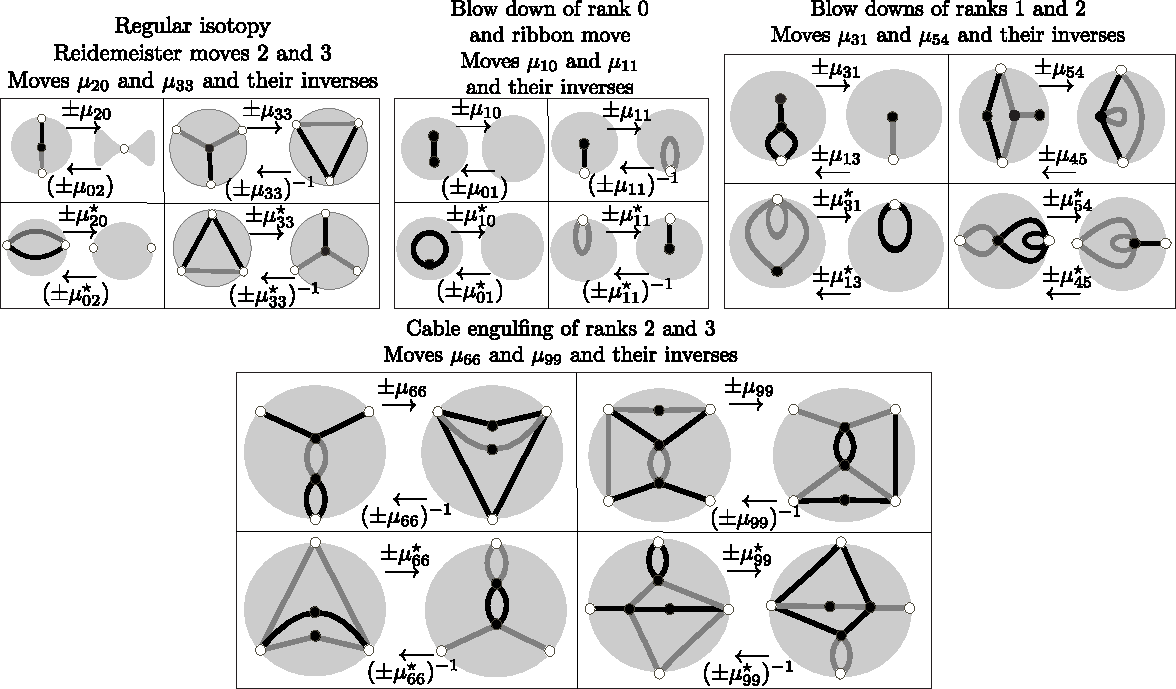
\includegraphics[width=16cm]{A.figs/blinkcalculus.pdf} 
  \end{center}
  \end{theorem}

 There are 64 local configurations of sub-blinks, each named a {\em coin}, 
 divided into 8 families of 8 simply related
 coins and also divided into 32 pairs of left-right coins,
  A move replaces the left (right) coin of a pair by its right (left) 
 coin. Thus, the number of moves is equal to the number of coins.
 Boundary and internal vertices of the coins are shown as small white disks. 
  The complementary sub-blink in the exterior a coin is completely arbitrary; 
 its intersection with the corresponding internal coin is a subset of the set of 
 attachment vertices in the boundary of the coin.
 The support of the coins
 are disks, except in the the right coin  
 of $\mu_{20}$, case in which is a pinched disk. 
 The number $k$ of the attachment vertices  satisfies $k\in \{0,1,2,3,4\}$. 
 A reduced but sufficient form of this coin 
 calculus having 36 coins (and moves) is obtained in the final section.

 \section{Motivation}
In his Appendix to part 0, J. H. Conway in his famous book {\em On Numbers and Games}, 
\cite{onnumbersandgames}, says: {\em ``This appendix is in fact a cry for a Mathematician
Liberation Movement!

Among the permissible kinds of constructions we should have:\\
(i) Objects may be created from earlier objects in any reasonable constructive fashion.\\
(ii) Equality among the created objects can be any desirable equivalence relation.''
} 
 
This paper is in the confluency of two deep research passions of the author, apparently very far apart:
the topological study of closed orientable 3-manifolds and the combinatorial study of plane 
graphs.  The result proved here provides a glimpse, in the spirit of 
Conway's quotation, to effectively
enumerate once each closed orientable 3-manifolds. 
Blinks are easy to construct from simpler blinks, and their 
isomorphism problem can be solved by a polynomial
algorithm which finds, via a few fixed conventions (lexicography), a numerical {\em code} for it. 
What can be more desirable than an equivalence relation on such simple mathematical 
objects that captures the subtle and difficult computational topological notion of
factorizing any homeomorphism between two closed, oriented, connected 3-manifolds?
 
\section{Topological preliminaries}

This section contains the basic topological material that I need. It is primarely intended to the 
combinatorially oriented readers, unfamiliar with the fundamental definitions of knots, 
links and framed lins.
The topological oriented readers also should read it 
because I introduce some unfamiliar notation and definitions which are new and that will be 
used throughout as well as  present a short historic overview of the known results.

\subsection{Links, framed links, blackboard framed links, bflink, blinks}

A {\em knot} is an embedding of a circle,  $\mathbb{S}^1$, into $\mathbb{R}^3$.
The {\em unknot} is a knot which is the boundary of a disk.
A {\em link with $k$ components} is an embedding of a disjoint union of $k$ 
copies of $\mathbb{S}^1$,
$\left(\cup_{i=1}^k \mathbb{S}^1_i \right)$,
into $\mathbb{R}^3$. In this way, a knot is a particular case of a link: one which
has one component.
A {\em framed link} is an embedding of 
$\left(\cup_{i=1}^k \mathbb{S}^1_i \right) \times [-\epsilon,+\epsilon]$  
into $\mathbb{R}^3$, for an arbitrarily fixed $\epsilon>0$. The {\em base link} of a framed
link is the framed link restricted to $\left(\cup_{i=1}^k \mathbb{S}^1_i \right) \times\{0\}$.  


Links can be presented with profit by their {\em decorated 
general position projections} into a fixed plane $\mathbb{R}^2$. {\em General position} means that 
in the image of the link there is no triple points and that at each neighborhood of
a double point is the transversal crossing of two segments of the link, named {\em strands}. 
{\em Decorated} means that we keep the information
of which strand is the upper one, usually by removing a piece of the lower strand. In this paper
I use yet another way to decorate the link projections: the images of the link components 
are thich black curves
and the upper strands are indicated by a thinner white segment inside the thich 
black curve at the crossing (see second definition in Fig. \ref{fig:somenotation}).


\begin{figure}[H]
\begin{center}
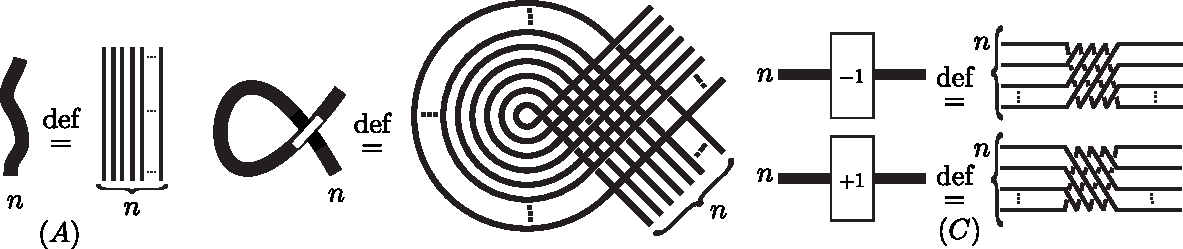
\includegraphics[width=16.5cm]{A.figs/somenotation.pdf} 
\caption{\sf Notation for special disk neighborhoods of general position decorated link projections}
\label{fig:somenotation}
\end{center}
\end{figure} 


The isotopy class of a framed link is determined by assigning an 
integer to each component of the link which is equal to the {\em linking number} of the
two components of the boundary of each of its bands oriented in the same way. The linking number 
can be obtained from an arbitrary decorated general position projection of the oriented band:
it is the algebraic sum of the $(\pm)$-signs of the crossings of distinct boundary components.
The convention is 
\raisebox{-3mm}{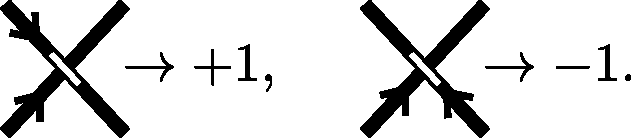
\includegraphics[width=3cm]{A.figs/plusoneminusonecrossing.pdf}}
The linking number is an invariant, that is, it does not depend on 
the particular projection used. This is proved by K. Reidemeister in its 1932 book
on Knot Theory, \cite{reid1932}. He isolates three local moves $r_1, r_2, r_3$ that
are enough to finitely factor any arbitrary ambient isotopy between two decorated general 
position projections of the same link:
\raisebox{-3mm}{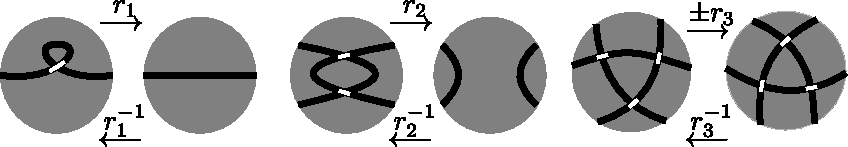
\includegraphics[width=7cm]{A.figs/reidemeistermoves.pdf}}.

As a matter of fact, Theorem \ref{theo:theorem} which 
I proved in this work is the counterpart for 3-manifolds
of Reidemeister Theorem. Note that in the coin calculus of depicted together
with bflinks in Fig. \ref{fig:blinkandlinktogether}
there are 8 versions of each of Reidemeister moves $r_2$ and $r_3$. Note also that 
Reidemeister move $r_1$ is not used at all. The equivalence class of bflinks generated
by $r_2^{\pm 1}$ and $r_3^{\pm 1}$ is called {\em regular isotopy}. It plays an important role
in the computation of the Jones invariants via Kauffman's bracket \cite{kauffman1987state}.

\begin{figure}[H]
\begin{center}

\includegraphics[width=8.5cm]{A.figs/GettingImmersedBandSameWidth.pdf} 
\caption{\sf Getting a constant width immersion of a band projection. 
Each 360-degree rotation of the band projection is ambient isotopic to
a curl in the band (in two different ways) so as to maintain  
constant the width immersion of the band projection.
In particular the images of
$\left(\cup_{i=1}^k \mathbb{S}^1_i \right) \times\{-\epsilon\}$,
and $\left(\cup_{i=1}^k \mathbb{S}^1_i \right) \times\{+\epsilon\}$
have 4 distinct points near each crossing of the base link.
}
\label{fig:GettingImmersedBandSameWidth}
\end{center}
\end{figure} 

A {\em blackboard framed link} is a projection of a framed link so that 
the base link is projected as a decorated general position one and its bands are immersed
with constant width $2\epsilon$. Moreover, we adjust the number of curls and their signs 
(in the base link) so that the framing of each component coincides with the linking number of 
the two boundary components of the band. The advantage of the blackboard framed link is that
we no longer have to worry about assigning numbers to the components. These numbers are induced
by the plane $\mathbb{R}^ 2$ of projection. The importance of this concept was 
advocated by L. Kauffman in a number of works, including \cite{kauffman1991knots} and 
\cite{kauffman1994tlr}. In this work, it is central: every framed link I use is presented as 
a {\em bflink}, defined as the base link of a blackboard framed link, with no numbers attached. 
Fig. \ref{fig:linkblink} shows a 1-1 correspondence between bflinks and blinks.

\begin{figure}[H]
\begin{center}
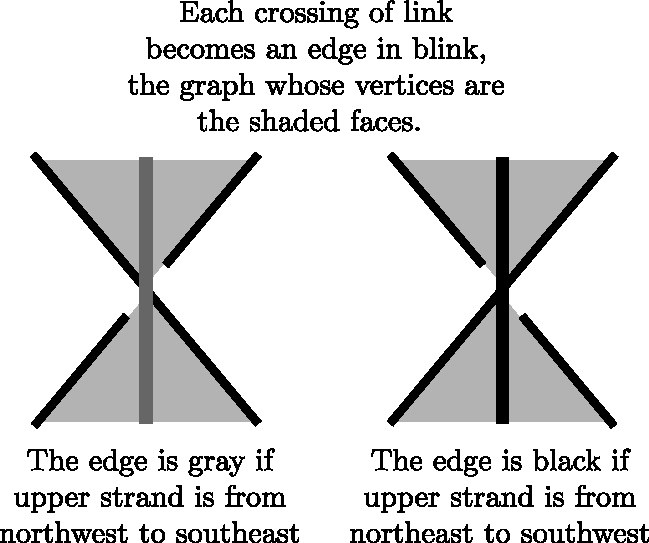
\includegraphics[width=15cm]{A.figs/linkblink.pdf} 
\caption{\sf From bflink to blink and back: 
the projection of any link can be 2-face colorable into white and gray with the infinite
face being white so that each subcurve between two crossing have their incident faces receiving distinct
colors. The above figure shows how to transform a link projection into a blink (with thicker edges
than the curves representing the link projection). 
The vertices of the blink are distinguished fixed
points represented by white disks in the interior of the gray faces. 
Each crossing of the link projection becomes an edge in the corresponding blink, 
An edge of the blink is gray if the upper strand 
that crosses it is from northwest to southeast, it is black if the the upper strand 
that crosses it is from northeast
to southwest. The inverse procedure
is clearly defined. In fact, the link is the so called {\em medial map} of the blink.
Thus we have a 1-1 correspondence between general position decorated link projections
and blinks. The (complete) blink at the right induces Poincar�'s sphere, 
the spherical dodecahedron space. The expressibility of a blink is powerful: quite
complicated 3-manifolds are induced by simple blinks.}
\label{fig:linkblink}
\end{center}
\end{figure} 

\subsection{Lickorish's groundbreaking result}
In a grounding breaking work (1962),  W.B.R. Lickorish, \cite{lickorish1962representation}, proved that
each closed orientable 3-manifold $\mathbb{M}^3$ can be encoded by a link in $\mathbb{S}^ 3$ 
where each one of its $k$ components
is endowed with an irreducible fraction (the framing) $\frac {\pm p}{q}$ 
where $q$ could be 0, and in the case $p$ must be 1 and the fraction
becomes $\pm \infty$. To construct $\mathbb{M}^3$ 
from the framed link I act as follows: after removing from $\mathbb{M}^3$
an $\epsilon$-neighborhood $(\mathbb{S}^ 1 \times \mathbb{D}^2)_i$ of the $i$-th link we are left with 
$\mathbb{M}^ 3\backslash \bigcup_{i=1}^k (\mathbb{S}^ 1 \times \mathbb{D}^2)_i=
\mathbb{S}^ 3\backslash \bigcup_{i=1}^k (\mathbb{S}^ 1 \times \mathbb{D}^2)_i$. The fraction specifies, in the 
toroidal boundary inside $\mathbb{S}^ 3$, the homology type $(\pm p,q)$ of the curve that
is contractible in the solid torus inside $\mathbb{M}^3$. For each component, we then
identify the simple curve given by the homological base pair with the meridian of a canonical copy of a 
solid torus in $\mathbb{R}^ 3$  so as to completely specify the pasting of the solid torus 
closing the toroidal hole.
Lickorish's breakthrough was to prove that any $\mathbb{M}^3$ has inside it a finite number
$k$ of disjoint solid tori so that $\mathbb{M}^ 3\backslash \bigcup_{i=1}^k 
(\mathbb{S}^ 1 \times \mathbb{D}^2)_i=
\mathbb{S}^ 3\backslash \bigcup_{i=1}^k (\mathbb{S}^1 \times \mathbb{D}^2)_i$.
Actually, this result had been proved 2 years before 
by A. H. Wallace \cite{wallace1960modifications} by using differential geometry. However
it was the purely topological flavor of Lickorish's proof that spurs the subsequent developments.

\subsection{Kirby's famous calculus of framed links}
In 1978 R. Kirby published his, to become famous, calculus of framed links, \cite{kirby1978calculus}.
The gist of this paper is that two types of moves 
are enough to go from any framed
link inducing a closed oriented 3-manifold to any other such link inducing the same manifold.
One of the moves is absolutelly local: creating or cancellating an arbitrary new unknotted 
component with frame $\pm 1$ separated from the rest of the link by an $\mathbb{S}�$.
The other type of move, {\em the band move}, \cite{kirby1978calculus, 
kauffman1991knots}) {\em (or handle sliding)} is non-local and infinite in number.

\begin{figure}
\begin{center}
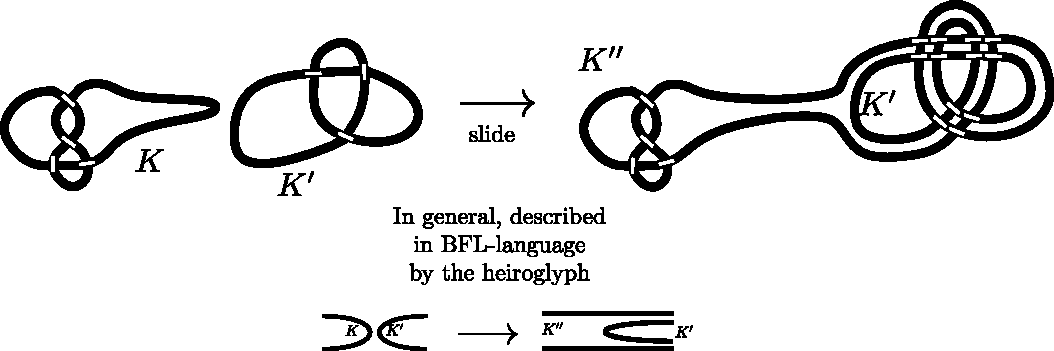
\includegraphics[width=14cm]{A.figs/handleslide.pdf} 
\caption{\sf Kirby's handle slide move, also known as the band move. Given $K$ and $K'$ two distinct components of a
link start by making a close parallel copy of $K'$ in such a way that it has linking number 0 with its originator $K'$.
Let $K''$ be the connected sum of $K$ and the copy of $K'$. The connected sum is defined by a {\em band} which is a
thin rectangle arbitrarily embedded into $\mathbb{S}^3$, so as to miss the link. 
The short sides of the band 
are attached to $K$ and to the copy of $K'$ and are recoupled in the other way.
The band can be quite complicated because it may wander
arbitrarily (as long as it misses the link) 
in $\mathbb{R}^3$ in its way to connecting
the two components. The situation loses no generality and becomes 
particularly simple if we have a bflink. 
More details in Kauffman's book, \cite{kauffman1991knots}. 
In bflink language, this move
is depicted in all its generality, via the hieroglyph shown in the bottom part of the 
Figure. See Section 12.3 of \cite{kauffman1994tlr}.}
\label{fig:handleslide}
\end{center}
\end{figure} 

\subsection{Fenn-Rourk reformulation of Kirby's calculus}
In 1979 R. Fenn and C. Rourke (\cite{fenn1979kirby}) show that Kirby's moves could 
be replaced by an infinite sequence of a single type of move (a {\em blow down move})
indexed by $n$, which I depict at the left side of Fig. \ref{fig:FennRourkeAndKauffmanMove}. 
In a blow down move the number of components decreases by 1.
This has been a very useful reformulation with many applications, 
including Martelli's calculus (soon to be treated)
which uses it instead of the direct moves of Kirby. 

\begin{figure}
\begin{center}
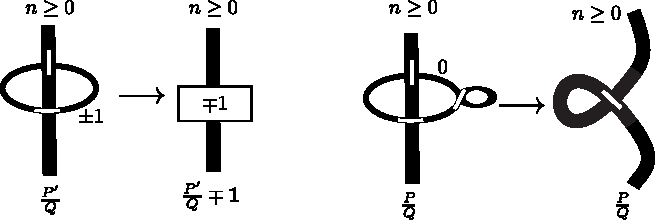
\includegraphics[width=13.5cm]{A.figs/FennRourkeAndKauffmanMove.pdf} 
\caption{\sf Fenn-Rourke infinite sequence of blown-down moves 
and their counterpart in Kauffman's blackboard framed links. These are
infinite sequence of local moves. Cases $n=0$ of these moves replace
an isolated $\pm 1$-framed component or the unknot with one crossing by nothing.
Martelli replaced the infinite sequence by the first three and two new simple
moves $A_3$ and $A_4$, described in Fig. \ref{fig:Martelli}.}
\label{fig:FennRourkeAndKauffmanMove}
\end{center}
\end{figure} 

\subsection{Kauffman's idea to let the plane induce the framing}
In the beginning of the 1990's L. Kauffman
presented (\cite{kauffman1991knots}) a completely planar diagramatic way to deal with the 
calculus of Kirby and its reformulation by Fenn and Rourke.
The basic idea comes from the fact that every 3-manifold is
induced by surgery on a framed link which has {\em only finite integer framings}. 
This characterize the {\em handle surgeries}. According to 
Rolfsen Lickorish call each of these a
{\em honest surgery}, page 262 of \cite{rolfsen2003knots}.
The proof that we can get any manifold by surgery on integer framed links 
uses, as a lemma,  the fact that it is possible to
modify the framed link maintaining the induced 3-manifold so that every component becomes unknotted. 
A proof of this lemma appears in Rolfsen's book. 
It also apears in page 137 of Kauffman-Lins monography,
\cite{kauffman1994tlr}. If a component is unknotted then 
it is simple to modify the link so that each component gets an integer framing, without 
distub the integrality of the framing of other components. So, without loss of
generality we may suppose that all the components have finite integers as framings. Kauffman's proceeds
by adjusting each component by attaching to it a judicious number of curls so that the required framing of
a component coincides with the algebraic sum of its self-crossings. 
By specifying that the link is {\em blackboard framed}, we no longer need the integers to
specifies the framing. They are a consequence.
In this work I only use links given by blackboard framed projections: 
they are rather close of blinks, which are purely graph theoretical plane graphs with 
an edge bipartition.

\subsection{Martelli's finite calculus on flinks}
In an important recent paper B. Martelli \cite{martelli2012finite} 
presented a local finite reformulation of
the Fenn-Rourke version (\cite{fenn1979kirby}) of Kirby's calculus \cite{kirby1978calculus}. 
This calculus is presented in Fig. \ref{fig:Martelli}. It remains
to be seen the consequences of Martelli' s result for obtaining new 3-manifold invariants.
A possible door for obtaining such invariants are generalizations of the combinatorial 
approach to get WRT-invariants, justified in \cite{kauffman1994tlr} and extensely
used in \cite{lins1995gca} and in \cite{lins2007blink}. To find such a generalization 
one has to take advantage of the specific sufficient local Martelli's moves now available 
(or the coin calculus on blinks) instead of 
hiding in the Temperley-Lieb algebra the infinite cases of Kirby's band move, 
as pioneered by Lickorish
in \cite{lickorish1991three}. See also page 144 of the join monography of 
L. Kauffman and myself, \cite{kauffman1994tlr}.

\begin{figure}
\begin{center}
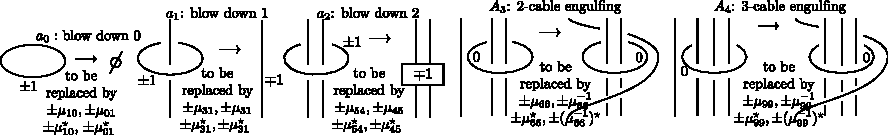
\includegraphics[width=16.5cm]{A.figs/Martelli.pdf} 
\caption{\sf Martelli's calculus on bflinks. 
He proves that by keeping only
the blown down of ranks 0, 1 and 2 and replacing all the remaining infinite sequence by two
new moves 2- and 3-cable engulfing (denoted by $A_3$ and $A_4$) a sufficient calculus for factorizing 
homeomorphisms between closed oriented and connected 3-manifolds is achieved solely in terms of blinks. 
Moves $A_3$ and $A_4$ do not translate into blink moves
because their left sides are disconnected. What makes this work possible is the replacement of
these non-connected configurations by equivalent moves $a_3$ and $a_4$ 
so that blink translations become available. 
See Fig. \ref{fig:proofequivalencea3A3a4A4} where the diagrams for the moves
appear -90$^{\tiny o}$-rotated relative to this Figure.
}
\label{fig:Martelli}
\end{center}
\end{figure} 

\section{Objective of the work}
Our objective here is to further reformulate Martelli's moves so as to obtain a calculus
of blinks, denominated {\em coin calculus}, 
which is an exact combinatorial counterpart for factorizing homeomorphisms of
closed, orientable, connected 3-manifolds. It has the consequence that each 3-manifold
becomes a subtle class of plane graphs. Our exposition is complete and elementary seeking
to reach both audiences: topologists and combinatorialists. We feel that this result may be interesting
for Combinatorics as well as to Topology and may enhance both areas: conceivably, some 
deep properties of plane graphs could be used to elucidate aspects of 
3-manifolds and vice-versa. 

Plane graphs are one of the most 
studied objects in Combinatorics. The role of planarity in finding polynomial efficient algorithm
is well established. For instance, the {\em Max Cut Problem},(\cite{garey1979computers}),
an NP-complete problem, becomes polynomial,
if the graph is in the plane. This was a consequence of J. Edmonds's optimal 
maximum matching theory polyhedral theory: \cite{Edmonds1965, edmonds1973matching}. 
Other NP-complete problems like the {\em Max Stable Vertex Set Problem}(\cite{garey1979computers}),
remain NP-complete when restricted to plane
graphs. Also well established is the
the role of plane graphs motivating and permitting useful generalizations 
in matroid theory, \cite{tutte1965lectures}.
Matroids are a source of polynomial algorithms. A. Lehman used this theory 
to provide a solution for the Shannon Switching Game \cite{lehman1964solution}. 
This solution was enhanced to a polynomial algorithm by J. Edmonds in \cite{edmonds1965lehman}.
Plane graphs and this paper were the motivation for his unexpected and amazing algorithm for polynomially 
finding a matroid partition into indepedent subsets, \cite{edmonds1968matroid}, with its 
various applications to scheduling problems. Yes, I do believe in {\em One Mathematics}, as advocated by 
L. Lovasz, in his famous essay, \cite{lovasz1998om}. The area of combinatorics, particularly
the area of efficient polynomial algorithms based on polyhedral methods had, ten years ago,
its maturity declared by means of the publication of its {\em Magnum Opus}, in three volumes with more than
1800 mathematically dense pages, by A. Schrijver, 
\cite{schrijver2003cop1, schrijver2003cop2, schrijver2003cop3}. It is my hope that
some aspects of the polyhedral theory may have consequences on 3-manifolds algorithmic theory.

Two interesting open questions relating plane graphs and 3-manifolds are: 
(1) Which 3-manifolds correspond to the class of 3-connected monochromatic blinks?
I have reasons to believe that the pair $\{$blink, dual blink$\}$ 
(and the associated $\{$graphic-cographic$\}$ matroids) 
is a complete invariant for these manifolds: a census of
all the 242 blinks which are $3$-connected, monochromatic 
and have up to 16 edges appear in \cite{lins2007blink}. In the domain of the census,
the pair $\{$graphical/cographical$\}$ matroids is a complete invariant.
(2) The theorem established in this work brings closer of being true an old quest of mine: 
is there a way to associate a matroidal invariant to a general closed, orientable and connected
3-manifold?

Eleven years ago, I. Agol, J. Hass and W. Thurston proved that {\em 3-manifold knot genus is NP-complete}, \cite{agol2002}.
There seems to be relatively few results along this line. This one in particular suffer from the fact
that it is very difficult to work combinatorially and to 
visualize a knot in an arbitrary 3-manifold. I think that
discovering more NP-complete problems in 3-manifolds could arise from the result here presented.
After all NP-complete problems abound in plane graphs. In my wildest dreams I see myself 
showing that reformulating one of these plane graph problem into the corresponding 
3-manifold problem is polynomially solvable by topological means.

\section{Proof of the Theorem}

\begin{figure}[H]
\begin{center}
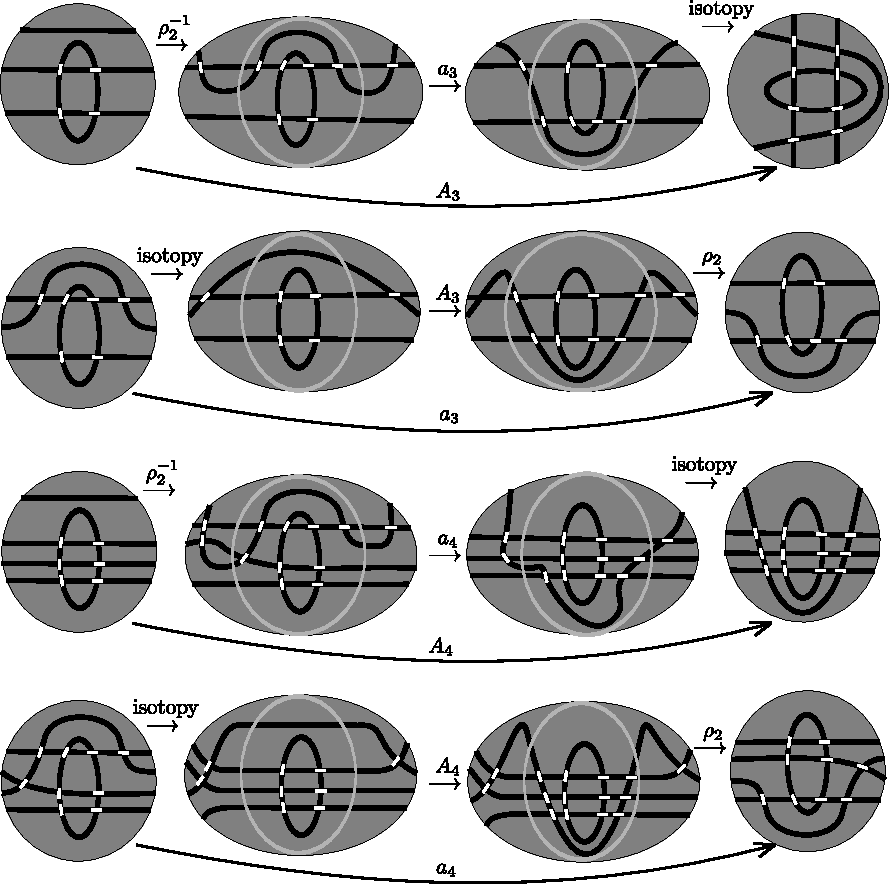
\includegraphics[width=14cm]{A.figs/proofequivalencea3A3a4A4.pdf} 
\caption{\sf A proof that in the presence of 
$\pm r_{2}^{\pm 1}$, the equivalences   
$a_3 \equiv A_3$ and $a_4 \equiv A_4$ hold}
\label{fig:proofequivalencea3A3a4A4}
\end{center}
\end{figure} 

\begin{lemma}
 In the presence of Reidemeister moves 2, generaly denoted by $\pm r_2^{\pm -1}$,
 moves $\pm a_3$ and $\pm A_3$ are equivalent and so are
 moves $\pm a_4$ and $\pm A_4$.
\end{lemma}
\begin{proof}
 We refer to  Fig. \ref{fig:proofequivalencea3A3a4A4}. Its first line proves that $\pm a_3 \Rightarrow \pm A_3$.
 The second line proves that $\pm A_3 \Rightarrow \pm a_3$. The third line proves 
 that $\pm a_4 \Rightarrow \pm A_a$. The last line proves that $\pm A_4 \Rightarrow \pm a_4$. 
\end{proof}

\begin{proof} ({\bf of Theorem \ref{theo:theorem}})\\
In Fig. \ref{fig:bflinkandlinktogether} we draw all the moves 
for the revised Martelli's moves on pairs of distinctly 2-colored bflinks 
and the respective blinks superimposed. The result follows by removing the 
bflink moves leaving solely the
blink moves which are shown again up to isotopy in the lower part of the figure.
\end{proof}


\begin{figure}[H]
\begin{center}
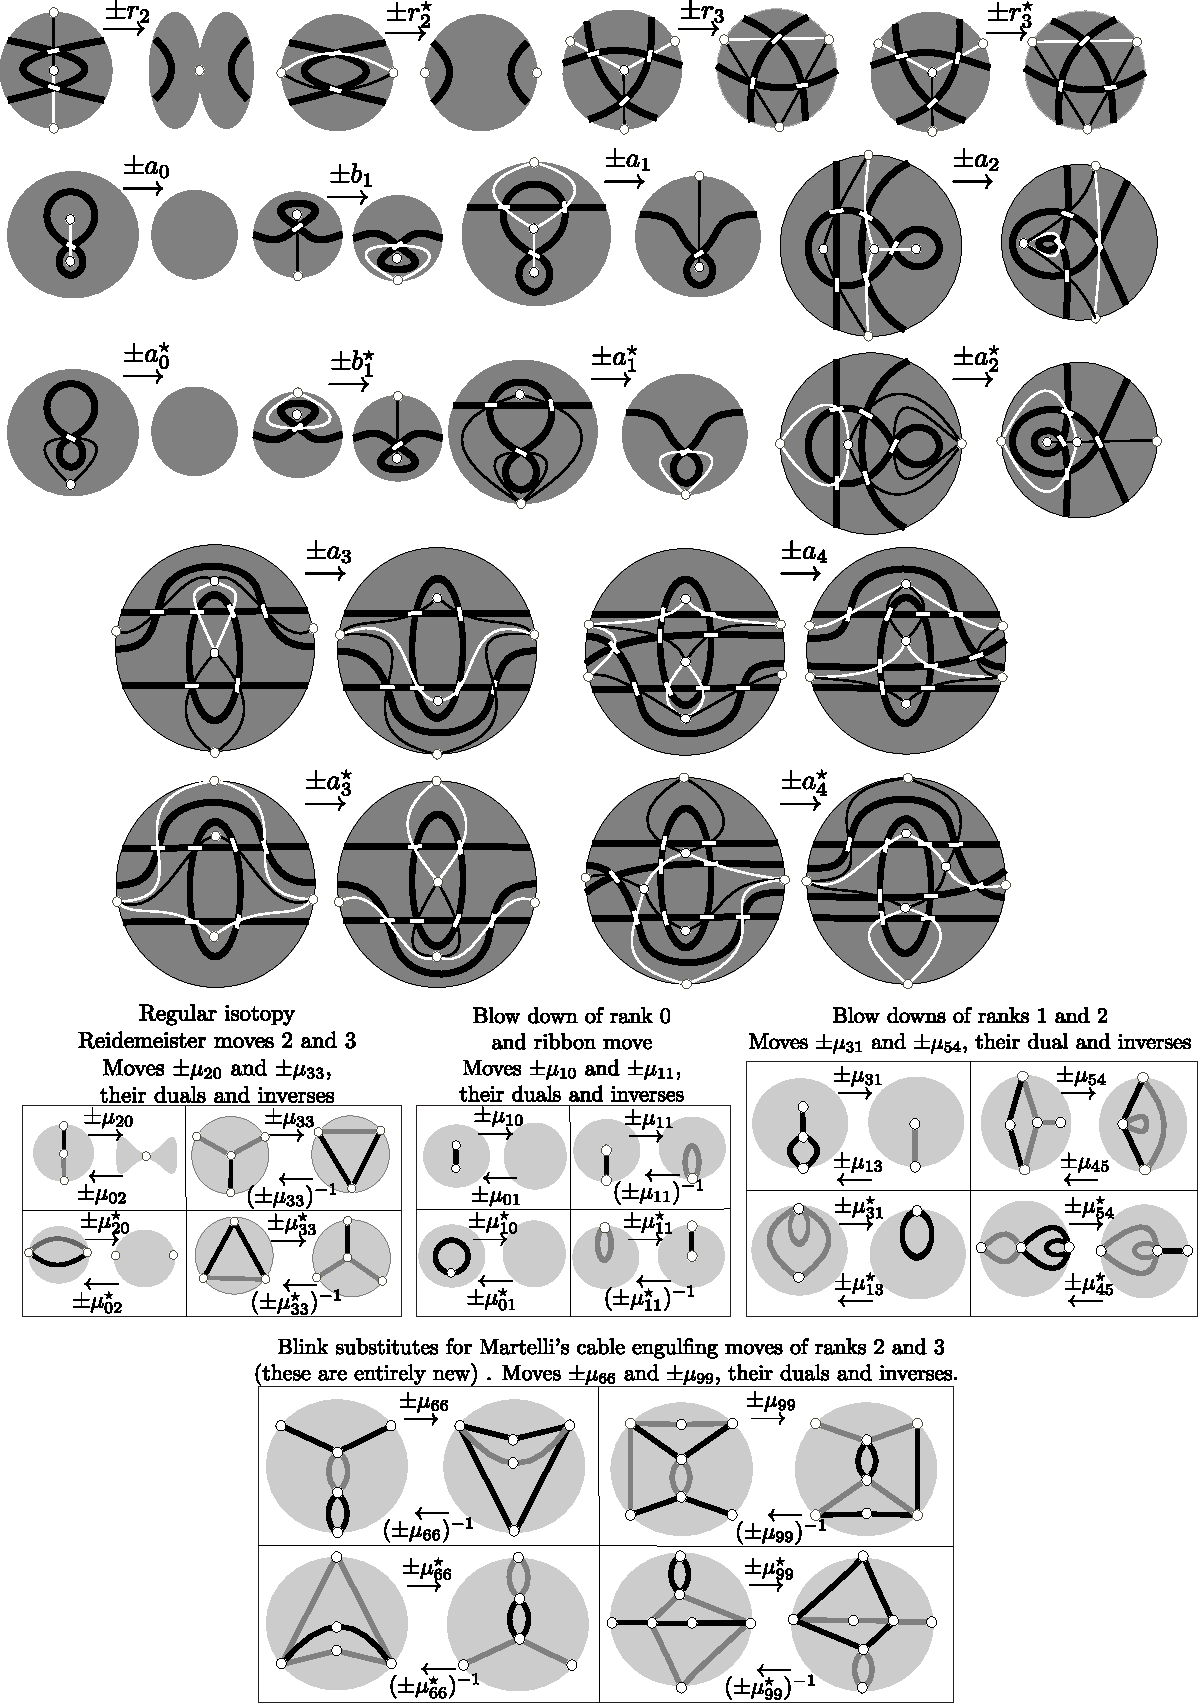
\includegraphics[scale=0.7]{A.figs/bflinkandlinktogether.pdf}
\caption{\sf Bflink version of Martelli's revised calculus with 
$a_3$, $a_4$ replacing $A_3$, $A_4$. 
In the upper part of the figure, distinctly 2-face colored bflinks 
and respective blinks are superimposed implying 
the moves for the coin calculus in the lower part of the figure, 
concluding the proof of the Theorem 1.1.}
\label{fig:bflinkandlinktogether}
\end{center}
\end{figure}

\section{The role of ribbon moves  $\pm \mu_{11}^{\pm 1}$}
The counterpart of the ribbon moves in the coin calculus, 
(also called ribbon moves) $\pm\mu_{11}^{\pm 1}$ are redundant 
because Martelli's calculus is in $\mathbb{R}^3$. We include them 
in our blackboard framed link calculus because with their inclusions all the dual moves,
except $\mu_{20}^\star$ and $\mu_{02}^\star$, become redundant.
\begin{corollary}
 The coin calculus can be simplified to include only the following set of 36 moves
 $ \{\pm \mu_{20}, \pm \mu_{02}, \pm \mu_{20}^\star, \pm \mu_{02}^\star, 
 \pm \mu_{33}^{\pm1}, \pm \mu_{01}, \pm \mu_{01},  \pm \mu_{11}^{\pm -1}, \pm \mu_{31},  \pm \mu_{13},  
 \pm \mu_{54},  \pm \mu_{45}, \pm \mu_{66}^{\pm},\pm \mu_{99}^{\pm}\}.$
\end{corollary}
\begin{proof}
 We work with the language of blackboard framed links which corresponds to the various coins.
 Moves corresponding to $(\pm \mu_{11}^{\pm1})^\star$ and  $(\pm \mu_{33}^{\pm1})^\star$ are redundant 
 because $\pm \mu_{11}^{\pm1}$  $\pm \mu_{33}^{\pm1}$ are self dual. 
 Moves $\pm\mu_{10}^\star$ and  $\pm\mu_{01}^\star$ are implied by a combination of moves 
 $\pm \mu_{10}$,  $\pm \mu_{01}$,  $\pm \mu_{11}$ and $(\pm \mu_{11})^{-1}$. 
 In particular, all the Reidemeister 2 and 3 moves (regular isotopy) 
 are at our disposal. We can use this fact to change the external face of
 the link diagram to become any chosen adjacent face by using regular isotopy at the cost of creating two 
 curls adjacent in the same component with distinct sign and the same rotation number. Use the the appropriate ribbon move to
 obtain two curls with the distinct signs and distinct rotation number. Now apply Whitney's trick
 (see page 30 of \cite{lins2007blink}) to cancel these curls. The net effect in the correponding 
 final blink  is that it is obtained from the initial blink by dualizing and interchanging black and gray
 edges. Having this double involutions at our disposal it
 is straighforward to obtain all the remaining dual moves.
\end{proof}
In Fig. \ref{fig:reducedblinkcalculus} I present the 36 moves of the final reduced coin calculus.
\begin{figure}[H]
\begin{center}
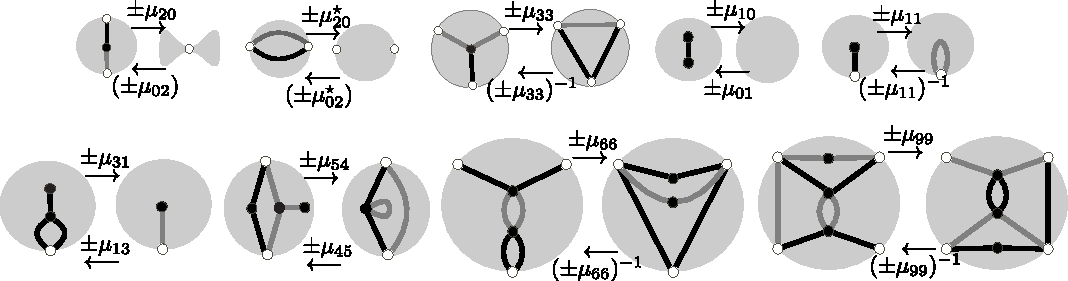
\includegraphics[scale=0.93]{A.figs/reducedblinkcalculus.pdf}
\caption{\sf The 36 moves forming the reduced coin calculus}
\label{fig:reducedblinkcalculus}
\end{center}
\end{figure}

\section{Conclusion}
I finished this work by presenting below a complete census of the $k$-small 3-manifolds, for $k=8$. 
These are the closed, oriented, connected and prime 3-manifolds 
induced by a blink with at most $k$ edges. 

\begin{figure}[H]
\begin{center}
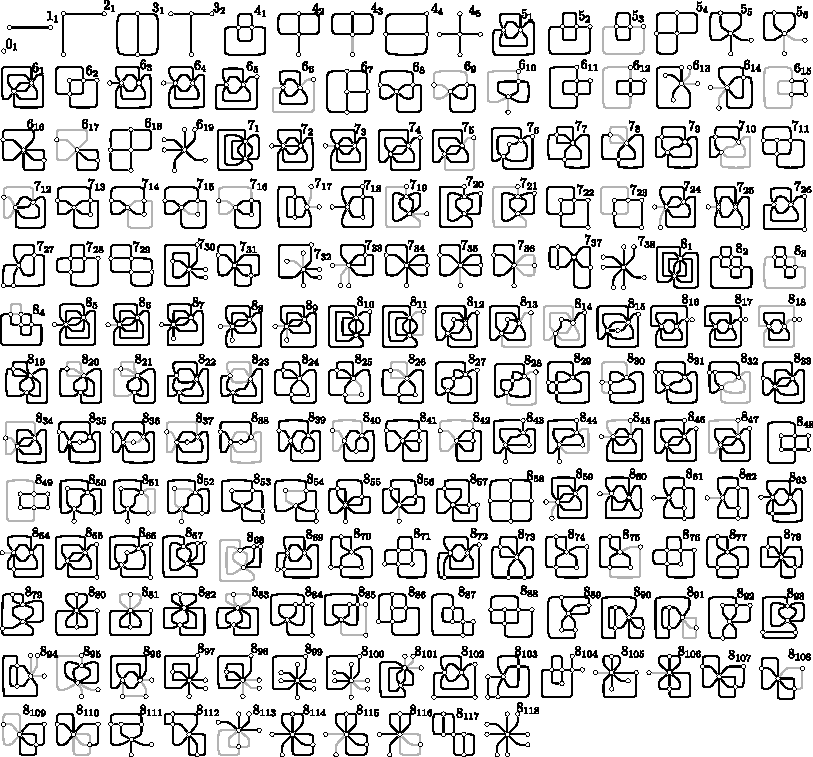
\includegraphics[scale=1.2]{A.figs/prime191Blinks-white-vertices.pdf}
\caption{\sf A complete census (no misses, no duplicates) of 8-small prime 3-manifolds. 
They correspond to the first 191 closed, oriented, connected and prime 3-manifolds. 
These are such 3-manifolds which are induced by blinks up to $k=8$ edges. 
A blink is a finite plane graph with an (arbitrary) edge bipartition. Such 
census are possible by completely combinatorial methods: we generate a subset of 
blinks that misses no 3-manifold by lexicography and the theory in \cite{lins2007blink};
then we compute the homology and the WRT-invariants; at this level $k=8$ 
these two invariants are seen to be complete. An entirely 
combinatorial recipe directly implementable to compute the WRT-invariants of a 3-manifold from 
a blink inducing it is given in Chapter 7 of \cite{lins1995gca}.
This recipe, in its turn is justified by at the very basic level, also by the combinatorial
theory developed in \cite{kauffman1994tlr}.}
\label{fig:prime191Blinks-white-vertices}
\end{center}
\end{figure}

%% \begin{figure}[!h]
% \begin{center}
% \includegraphics[width=12.5cm]{A.figs/seconddoubtB.pdf}
% \caption{\sf Finding presentations for the fundamental groups of $M^ 3[2125]$ and $M^ 3[2165]$}
% \label{fig:seconddoubtB}
% \end{center}
% \end{figure}

%-----------------------------------
\bibliographystyle{plain}
%\bibliographystyle{is-alpha}
%\addcontentsline{toc}{bibliografia}{\MakeTextUppercase{Referências Bibliográficas}}
%\bibliography{d:/slsl\3.DadosSostenes.35.ArtigosLivros.bibtexGoogleScholar/bibtexIndex.bib} % bib file is slsl.bib
%\bibliography{~/home/ricardo/Dropbox/35.ArtigosLivros.bibtexGoogleScholar/bibtexIndex.bib}
\bibliography{bibtexIndex.bib}
%\bibliography{slsl}


\vspace{5mm}
\begin{center}
\hspace{7mm}
\begin{tabular}{l}
   S\'ostenes L. Lins\\
   Centro de Inform\'atica, UFPE \\
   Av. Jornalista Anibal Fernandes s/n\\
   Recife, PE 50740-560 \\
   Brazil\\
   sostenes@cin.ufpe.br
\end{tabular}


\end{center}


-----------------------------------
\bibliographystyle{plain}
%\bibliographystyle{is-alpha}
%\addcontentsline{toc}{bibliografia}{\MakeTextUppercase{Refer�ncias Bibliogr�ficas}}
%\bibliography{d:/slsl\3.DadosSostenes.35.ArtigosLivros.bibtexGoogleScholar/bibtexIndex.bib} % bib file is slsl.bib
%\bibliography{~/home/ricardo/Dropbox/35.ArtigosLivros.bibtexGoogleScholar/bibtexIndex.bib}
\bibliography{bibtexIndex.bib}
%\bibliography{slsl}


\vspace{5mm}
\begin{center}
\hspace{7mm}
\begin{tabular}{l}
   S\'ostenes L. Lins\\
   Centro de Inform\'atica, UFPE \\
   Av. Jornalista Anibal Fernandes s/n\\
   Recife, PE 50740-560 \\
   Brazil\\
   sostenes@cin.ufpe.br
\end{tabular}


\end{center}


\end{document}

% \printindex